%_____________________________________________________________________________________________ 
% Chapter 4: System Design
%_____________________________________________________________________________________________ 
\chapter{System Design}
\label{sec:system_design}

Our design is modular by necessity.  Each of the four issues touches a different part of the
system, so we treat them as separate modules that plug into a shared consensus core.
Fig.~\ref{fig:architecture} shows how the pieces fit together.

\begin{figure}[t]
\centering
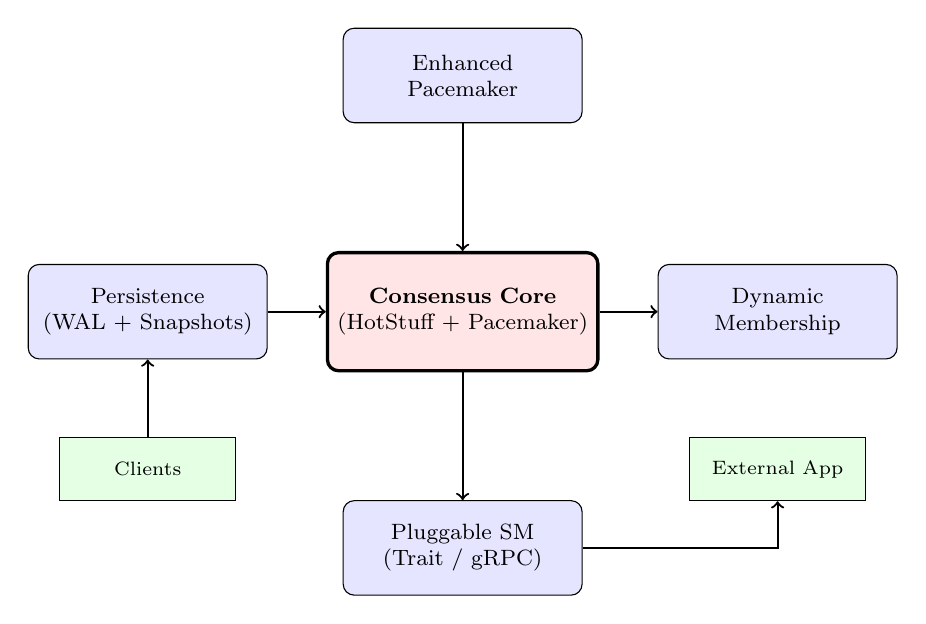
\begin{tikzpicture}[node distance=1.5cm, auto]
\tikzstyle{module}=[rectangle, draw, fill=blue!10, text width=2.8cm,
  text centered, minimum height=1.2cm, rounded corners,
  font=\footnotesize]
\tikzstyle{core}=[rectangle, draw, fill=red!10, text width=3.2cm,
  text centered, minimum height=1.5cm, rounded corners, very thick,
  font=\footnotesize]
\tikzstyle{interface}=[rectangle, draw, fill=green!10, text width=2cm,
  text centered, minimum height=0.8cm, font=\scriptsize]
\tikzstyle{arrow}=[->, thick]

\node (core) [core]
  {\textbf{Consensus Core}\\(HotStuff + Pacemaker)};
\node (persistence) [module, left of=core, xshift=-2.5cm]
  {Persistence\\(WAL + Snapshots)};
\node (membership) [module, right of=core, xshift=2.5cm]
  {Dynamic\\Membership};
\node (app_interface) [module, below of=core, yshift=-1.5cm]
  {Pluggable SM\\(Trait / gRPC)};
\node (liveness) [module, above of=core, yshift=1.5cm]
  {Enhanced\\Pacemaker};

\draw [arrow] (persistence) -- (core);
\draw [arrow] (core) -- (membership);
\draw [arrow] (core) -- (app_interface);
\draw [arrow] (liveness) -- (core);

\node (client) [interface, below of=persistence, yshift=-0.5cm]
  {Clients};
\node (application) [interface, below of=membership, yshift=-0.5cm]
  {External App};

\draw [arrow] (client) -- (persistence);
\draw [arrow] (app_interface.east) -| (application);
\end{tikzpicture}
\caption{High-level architecture.  Solid arrows show data flow.}
\label{fig:architecture}
\end{figure}

%-----------------------------------------------------------------------------
\section{Persistence Layer (WAL + Snapshots)}
\label{sec:persistence}

The idea is to write every state-changing event to an append-only log \emph{before} updating
the in-memory state, and periodically take a full snapshot so the log can be truncated.
What makes the Byzantine setting different is that a recovering replica cannot blindly trust
what it reads off disk.  A corrupted disk block or a Byzantine operator who tampered with
the log file must be detected, not silently absorbed.  So every WAL entry carries a CRC32
checksum, and the file header includes a SHA-256 digest of its own fields.

Tables~\ref{tab:wal-header} and~\ref{tab:wal-entry} show the binary layout.  We keep it
simple; there is no need for a complex log-structured storage engine here, since the WAL is
strictly append-only and reads happen only during recovery.  Sizes in
Table~\ref{tab:wal-header} are in bytes.

\begin{table}[t]
\centering
\setlength{\tabcolsep}{3pt}
\renewcommand{\arraystretch}{1.05}
\begin{tabular}{r r l p{4.5cm}}
\hline
\textbf{Offset} & \textbf{Size} & \textbf{Field} & \textbf{Description} \\
\hline
0  & 4  & Magic Number    & 0x48534C57 (``HSLW'') \\
4  & 2  & Version         & Format version (currently 0x0001) \\
6  & 8  & Replica ID      & Owner of this log \\
14 & 8  & Created Time    & Unix timestamp (ms) \\
22 & 32 & Header Checksum & SHA-256 over the preceding fields \\
\hline
\end{tabular}
\caption{WAL file header layout.}
\label{tab:wal-header}
\end{table}

\begin{table}[t]
\centering
\setlength{\tabcolsep}{4pt}
\renewcommand{\arraystretch}{1.1}
\begin{tabular}{|p{8cm}|}
\hline
\centering \textbf{Entry Frame} \\
\hline
Length (4\,B) \quad CRC32 (4\,B) \quad Payload (variable) \\
\hline
\end{tabular}
\caption{Each WAL entry is length-prefixed and checksummed.}
\label{tab:wal-entry}
\end{table}

Every entry is \texttt{fsync}'d before the corresponding in-memory update proceeds.  This
means a crash at any point leaves the log in a recoverable state: either the entry was fully
written (and its checksum will match), or it was not (and recovery will detect the
truncation).

\smallskip\noindent\textbf{Snapshots.}\quad
If left unchecked, the WAL would grow without bound.  We take a snapshot every $N$ committed
commands ($N{=}1000$ in our tests) capturing the block tree, committed log,
\texttt{high\_qc}, and eventually the application state.  Once a snapshot succeeds, all WAL
entries before its sequence number can be safely deleted.  Snapshots are serialised with
\texttt{bincode} via \texttt{serde}, which gives us compact binary output without the
overhead of a text format.

\smallskip\noindent\textbf{Recovery.}\quad
The procedure is straightforward (Algorithm~\ref{alg:wal_recovery}): load the most recent
snapshot, replay any WAL entries that came after it, verify each entry's checksum, and
rejoin the protocol.  If a checksum fails, the replica halts rather than risk operating on a
corrupted state; this is a deliberate choice.  In a Byzantine setting it is better to stop
and ask for help than to silently diverge from the rest of the quorum.

\begin{algorithm}[t]
\caption{Recovery from snapshot + WAL}
\label{alg:wal_recovery}
\begin{algorithmic}[1]
\REQUIRE Snapshot store, WAL store
\ENSURE Recovered replica state
    \STATE $\textit{snap} \gets \textsc{LoadSnapshot}()$
    \STATE $\textit{state} \gets \textsc{Restore}(\textit{snap})$
    \STATE $\textit{entries} \gets \textsc{LoadWAL}(\textit{snap.seqNo})$
    \FORALL{$\textit{entry} \in \textit{entries}$}
        \IF{$\textsc{VerifyCRC}(\textit{entry})$}
            \STATE $\textsc{Apply}(\textit{state}, \textit{entry})$
        \ELSE
            \STATE \textbf{halt} with error
        \ENDIF
    \ENDFOR
    \RETURN \textit{state}
\end{algorithmic}
\end{algorithm}

%-----------------------------------------------------------------------------
\section{Dynamic Membership}
\label{sec:membership}

Static validator sets are a real operational headache.  If a node dies permanently, you are
stuck with reduced capacity.  If you want to scale up, you need to restart everyone.  We
propose handling membership changes \emph{through the consensus protocol itself}, which
avoids introducing a separate coordination mechanism.

The idea is simple enough: a \texttt{JoinValidator} or \texttt{RemoveValidator} command is
included in a block like any other client request.  It flows through proposal, voting, and
QC formation normally.  The membership change only takes effect once the enclosing block is
committed via the 3-chain rule.  This gives us atomicity for free; either the change commits
or it does not, and all honest replicas agree on which blocks were committed.

For joins, the new replica would need to catch up by downloading the latest snapshot and
replaying subsequent WAL entries from an existing peer.  For removals, the departing replica
simply stops participating after the commit.

One subtlety we want to flag: quorum intersection across configurations.  In a single
configuration, any two quorums of size $2f{+}1$ out of $3f{+}1$ must overlap in at least
one honest replica.  When the configuration changes, we need to make sure decisions made
under the old quorum are respected by the new one.  Our approach is to apply the change
atomically \emph{after} commitment, so the finalised chain prefix is locked in under the old
configuration's quorum rules before the new configuration activates.  We formally verify
this property and six additional membership safety invariants via exhaustive TLC model
checking (see Section~\ref{sec:formal_verification}).

%-----------------------------------------------------------------------------
\section{Pluggable State Machine}
\label{sec:pluggable_sm}

Most HotStuff prototypes just append commands to a log and call it a day.  We want the
consensus layer to be oblivious to what it is ordering---whether it is a key-value store, a
counter, a blockchain ledger, or whatever the application needs.

Our design defines a Rust \texttt{App} trait with three methods: \texttt{apply(cmd)} to
execute a command, \texttt{snapshot()} to capture application state, and
\texttt{restore(state)} to rebuild it.  This is directly inspired by Tendermint's
ABCI~\cite{tendermint}; we make no claim of novelty on the interface itself.  The value is
in integrating it cleanly with the WAL/snapshot machinery described above.

For applications that are not written in Rust, we plan to expose the same three operations
over gRPC~\cite{grpc}: an \texttt{Execute} RPC replaces \texttt{apply}, and
\texttt{Snapshot}/\texttt{Restore} RPCs handle state persistence.  We have also considered
WASM as an alternative for sandboxing untrusted plugins, though that remains speculative at
this point.

%-----------------------------------------------------------------------------
\section{Enhanced Pacemaker}
\label{sec:pacemaker}

The liveness problem under low load is subtle but annoying.  Say a client submits one
command.  The leader wraps it in a block and gets a QC.  However, the 3-chain rule means
that the block will not commit until two more QC-justified blocks appear after it.  If no
more client commands arrive, those blocks never get proposed, and the original command sits
in limbo indefinitely.

Our fix is for the pacemaker to monitor two conditions: (a)~has it been longer than
\texttt{timeout\_ms} since the last proposal? and (b)~are there fewer than three pending
blocks?  If both hold and the client queue is empty, the leader proposes a \emph{dummy
block}---a block with a no-op command.  Dummies go through the full consensus path
(proposal, vote, QC) and fill out the 3-chain.  At the application layer, they are simply
ignored.

The focus is wiring it into HotStuff's pacemaker correctly so that (a)~dummies do not
starve real commands, and (b)~the commit latency for a single command is bounded by roughly
$3 \times \textit{timeout}$.

%-----------------------------------------------------------------------------
\section{Consensus Core}

The algorithm for the core consensus protocol was described in
Chapter~\ref{sec:background}.  Given below are the core data structures used to implement
it.

\subsection{Blocks and the Block Tree}

Each block is a tuple
$B = \langle \mathit{hash},\ \mathit{parent},\ \mathit{view},\ \mathit{proposer},\
\mathit{qc},\ \mathit{cmds} \rangle$.
Blocks form a tree rooted at a genesis block; we store it as a
\texttt{BTreeMap<Hash, Block>} for $O(\log n)$ lookups.

\subsection{Cryptographic Authentication}

We use Ed25519~\cite{ed25519} throughout.  Each replica generates its own signing key at
startup and publishes the corresponding verifying key to all peers.  Votes are signed over
$\texttt{SHA-256}(\mathit{block\_hash} \| \mathit{view})$, and a QC requires $\ge 2f{+}1$
valid signatures from distinct replicas.  We chose Ed25519 over, say,
Boneh--Lynn--Shacham (BLS) because it is fast, widely supported, and the
\texttt{ed25519-dalek} crate is mature.

\subsection{Voting and QC Formation}

A replica votes for a proposal if: the proposer is the legitimate leader for that view, the
parent block exists locally, and any embedded QC verifies.  We also reject duplicate
votes---same signer, same block.  Once the leader accumulates $\ge 2f{+}1$ valid votes, it
assembles a QC.

\subsection{Commit Rule}

Algorithm~\ref{alg:commit} formalises what happens: for every uncommitted block $B_0$, we
look for a child $B_1$ and a grandchild $B_2$, both QC-justified.  If the chain exists,
$B_0$ commits.  In practice, commits happen at the speed of proposal rounds.

\begin{algorithm}[t]
\caption{3-chain commit detection}
\label{alg:commit}
\begin{algorithmic}[1]
\REQUIRE Block tree $\mathcal{T}$, committed set $\mathcal{C}$
\ENSURE Updated $\mathcal{C}$
\FORALL{$B_0 \in \mathcal{T} \setminus \mathcal{C}$}
    \STATE $B_1 \gets \textsc{Child}(\mathcal{T}, B_0)$
    \IF{$B_1 = \bot$ \textbf{or} $B_1.\mathit{qc} = \bot$}
        \STATE \textbf{continue}
    \ENDIF
    \STATE $B_2 \gets \textsc{Child}(\mathcal{T}, B_1)$
    \IF{$B_2 = \bot$ \textbf{or} $B_2.\mathit{qc} = \bot$}
        \STATE \textbf{continue}
    \ENDIF
    \STATE $\mathcal{C} \gets \mathcal{C} \cup \{B_0\}$
\ENDFOR
\RETURN $\mathcal{C}$
\end{algorithmic}
\end{algorithm}

\subsection{Leader Rotation}

Nothing fancy: $\textit{leader}(v) = v \bmod n$.  If a view times out, replicas increment
their view number and move on.  We may explore reputation-based rotation later, but
round-robin is fine for now.
